\documentclass[../poliXuniversity_hospital_(USP)_report.tex]{subfiles}


\begin{document}
\chapter{Hardware Golgi}

Apos muita pesquisa, analise das soluções disponíveis no mercado e discussões com professores e parceiros do HU, foi determinado os requisitos que o equipamento deveria satisfazer. De maneria sucinta, o equipamento deveria ter mecanismos que fosse capaz de armazenar remedios unitarizados, captura-los e dispensá-los de maneira rápida e confiavel, além disso a máquina deve possuir uma estrutura e segura em termos eletromecânicos e sanitários. 

\begin{figure}[h]
\centering
\caption{Estrutura Golgi Bot}
    \begin{minipage}{0.5\textwidth}
       \centering
        
        \centering % para centralizarmos a figura
        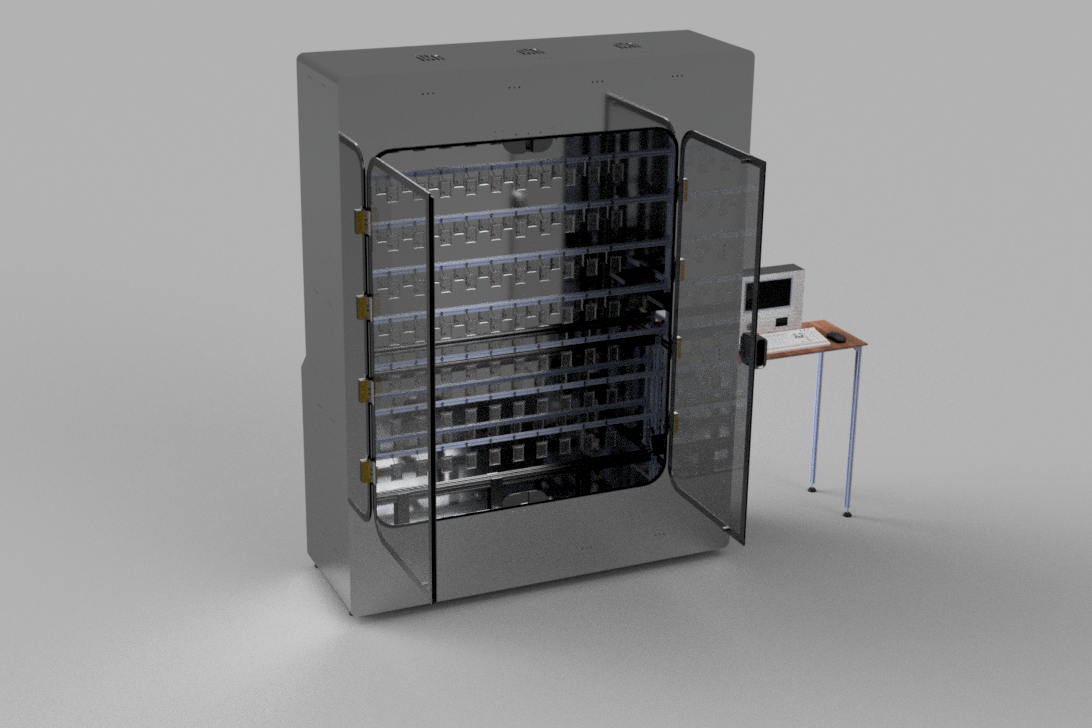
\includegraphics[width=7cm]{images/estrutura_golgi.png}
        
        
    \end{minipage}\hfill
    \begin{minipage}{0.5\textwidth}
        \centering
        \centering % para centralizarmos a figura
        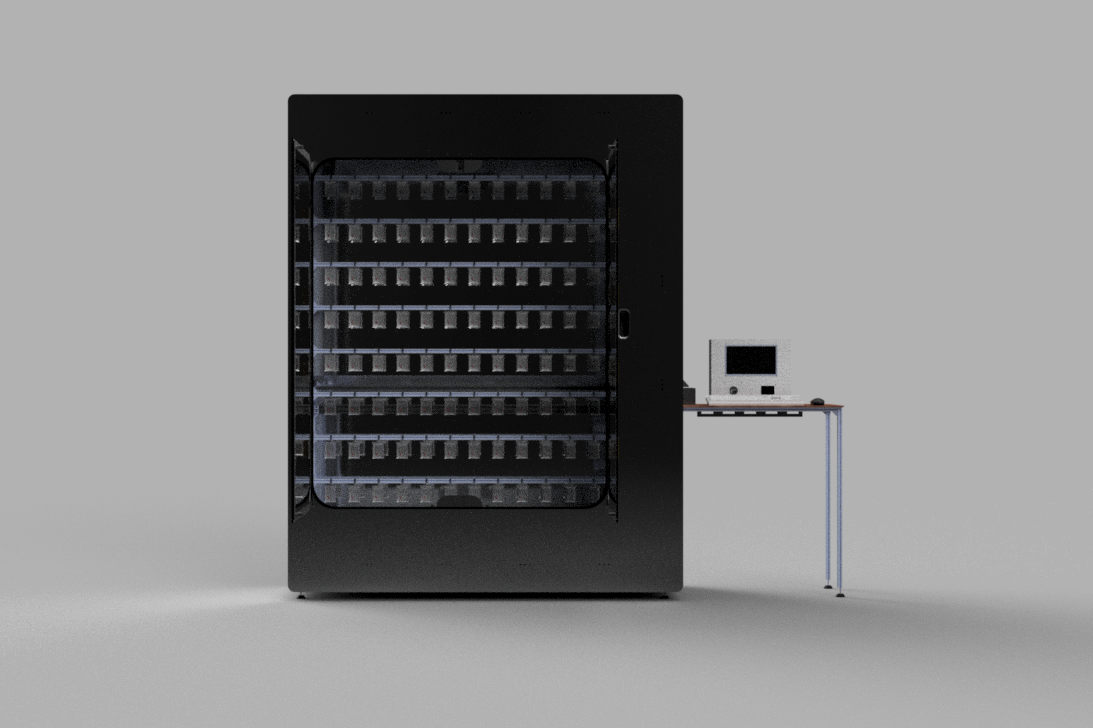
\includegraphics[width=7cm]{images/estrutura_golgi_1.png}
    \end{minipage}\hfill
    \caption*{Fonte: Autor}
    \label{figura: Estrutura Golgi Bot}
\end{figure}

\section{Estrutura Mecânica}


\subsection{Armazenamento de fármacos}
Inspirado em "vending machines", os remédios serão dispostos em cabides. Tais capides possuem angulação ideal e contra peso para garantira captura dos pacotes. Os cabides e contra pesos foram modelados e manufaturados no laboratório da equipe. Com 96 cabides cada um podendo armazenar cerca de 10 pacotes unitarizados a capacidade total seria de 960 comprimidos quanto completamente cheio.

\begin{figure}[h]
\centering
\caption{Cabide de remédios Golgi Bot}
    \begin{minipage}{0.5\textwidth}
       \centering
        
        \centering % para centralizarmos a figura
        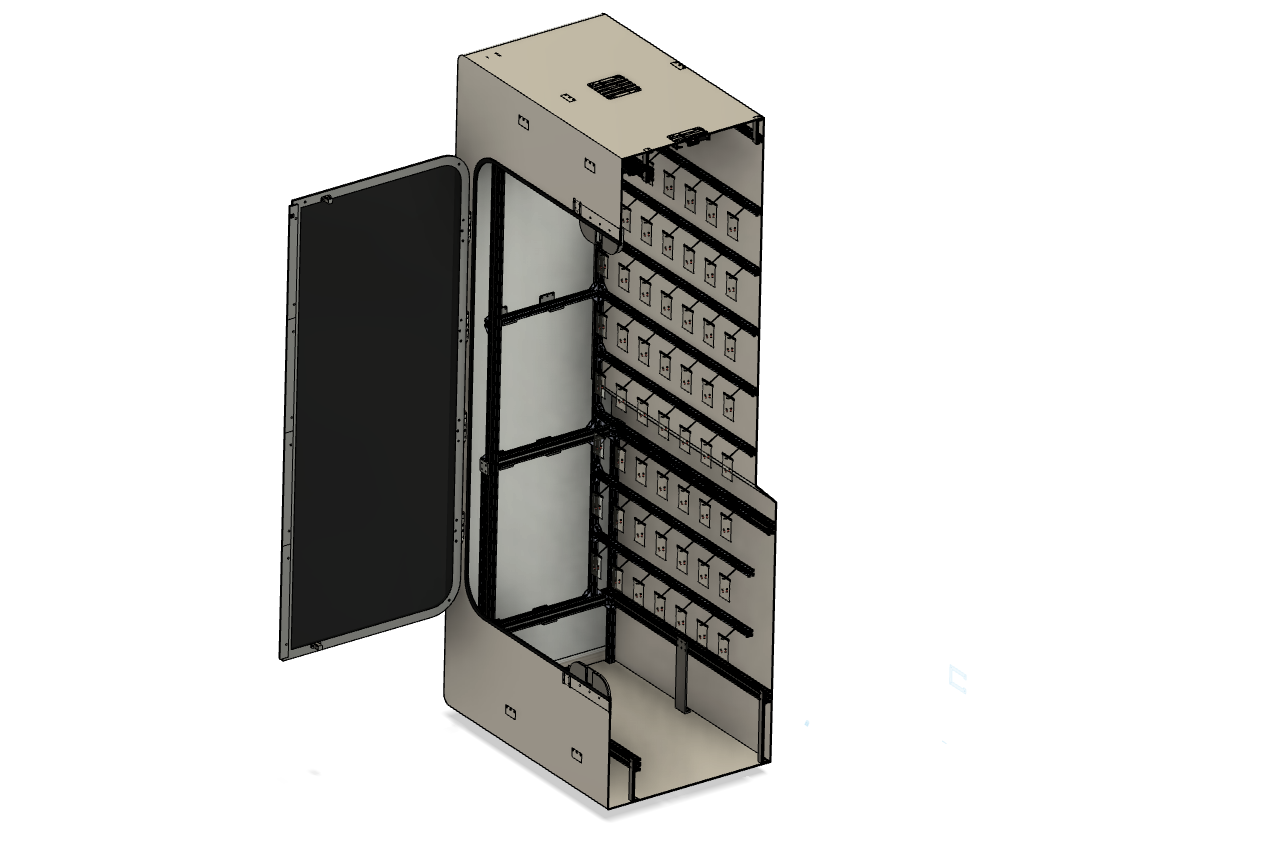
\includegraphics[width=7cm]{images/angulada_cabide.png}
        
        
    \end{minipage}\hfill
    \begin{minipage}{0.5\textwidth}
        \centering
        \centering % para centralizarmos a figura
        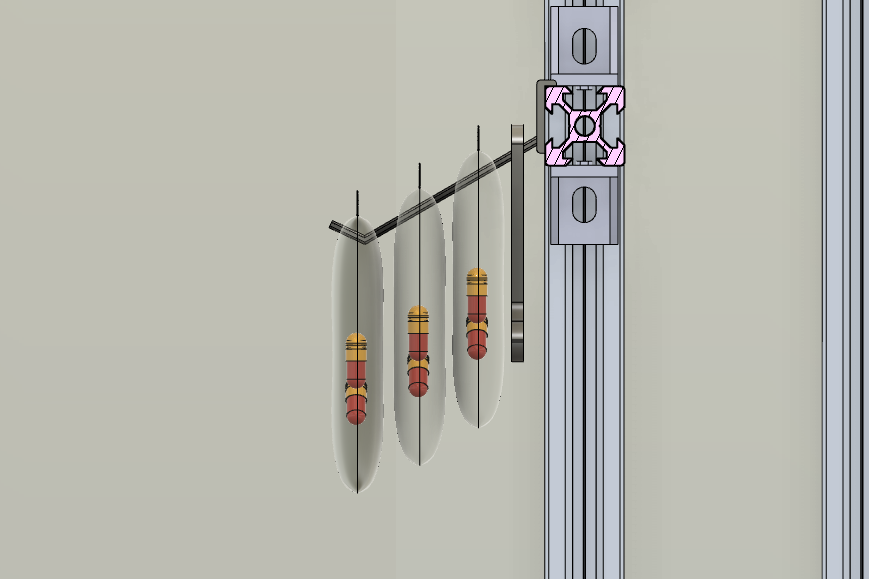
\includegraphics[width=7cm]{images/lateral_cabide.png}
    \end{minipage}\hfill
    \caption*{Fonte: Autor}
    \label{figura: Estrutura Golgi Bot}
\end{figure}

\subsection{Mecanismo de movimentação 3D}

Para que cada remedio consiga ser selecionado, foi desenvolvido um mecanismo de movimentação com 3 graus de liberdade com uma venotsa de sucção em sua extremidade. Foram usados rodizios de rolamento para perfil V-slot, solução inspirada em CNCs e impressoras 3D que utilizam o mesmo mecanismo para sua movimentação. Esse mecanismo possibilida posicionar nosso apanhador de remedios em qualquer posição XY de nosso cabiderio de remédios


\begin{figure}[h]
\centering
    \begin{minipage}{0.5\textwidth}
       \centering
        \caption{Roldanas V-SLOT Golgi bot}
        \centering % para centralizarmos a figura
        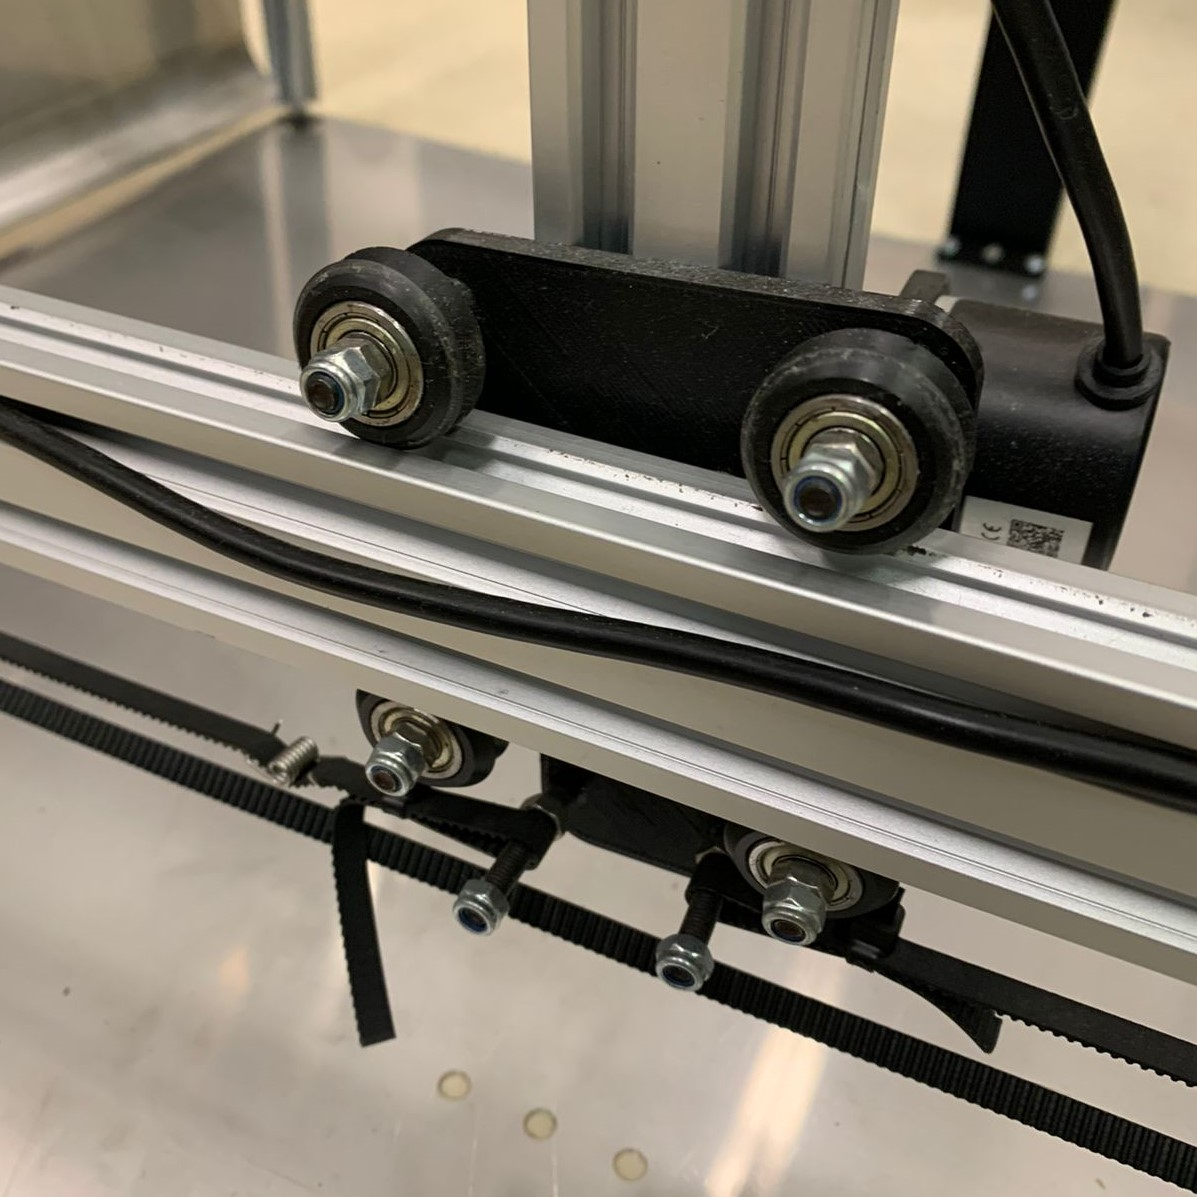
\includegraphics[width=7cm]{images/roldada_golgi.jpeg}
        \label{figura: Roldanas V-SLOT Golgi bot}
    \end{minipage}\hfill
    \begin{minipage}{0.5\textwidth}
        \centering
        \caption{Roldanas V-SLOT Creality CR-10 PRO}
        \centering % para centralizarmos a figura
        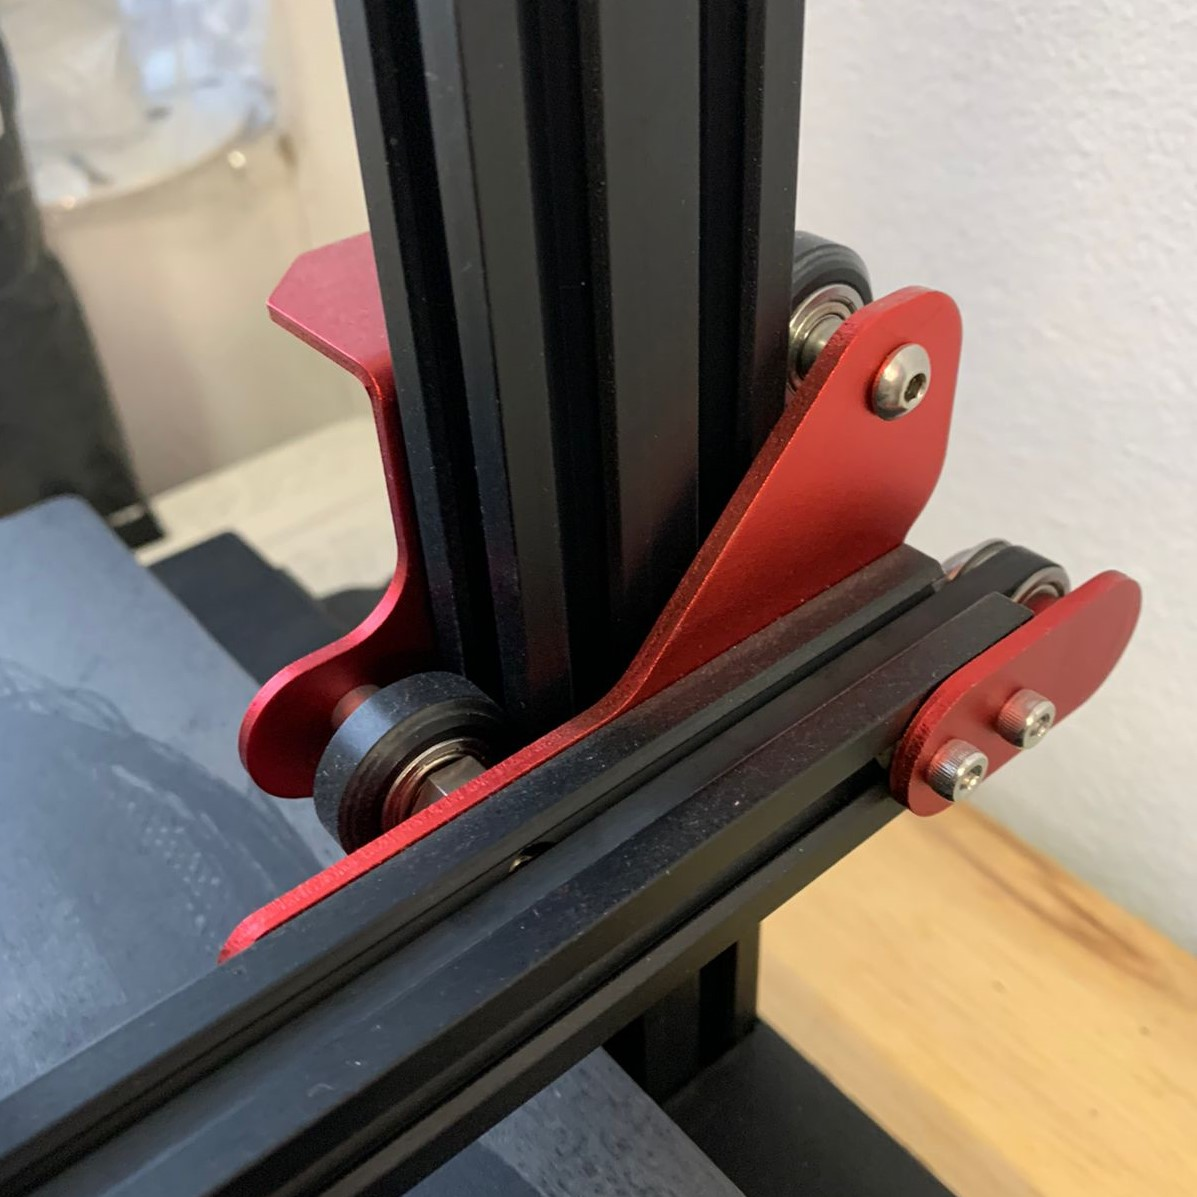
\includegraphics[width=7cm]{images/roldanacr10.jpeg}
        \label{figura: Roldanas V-SLOT Creality CR-10 PRO}
    \end{minipage}\hfill
    \caption*{Fonte: Autor}
\end{figure}
Para tracionar a movimentação em XZ foram usados motores12V 800RPM que utilizam um estagio de redução (4:1). Foram alocados dois motores para tração em X e um para Y e correias dentadas GT2 para transmissão do torque para o eixo Y e para o apanhador.

\begin{figure}[h]
\centering
    \begin{minipage}{0.5\textwidth}
        \centering
        \caption{Esquema de Tração}
        \centering % para centralizarmos a figura
        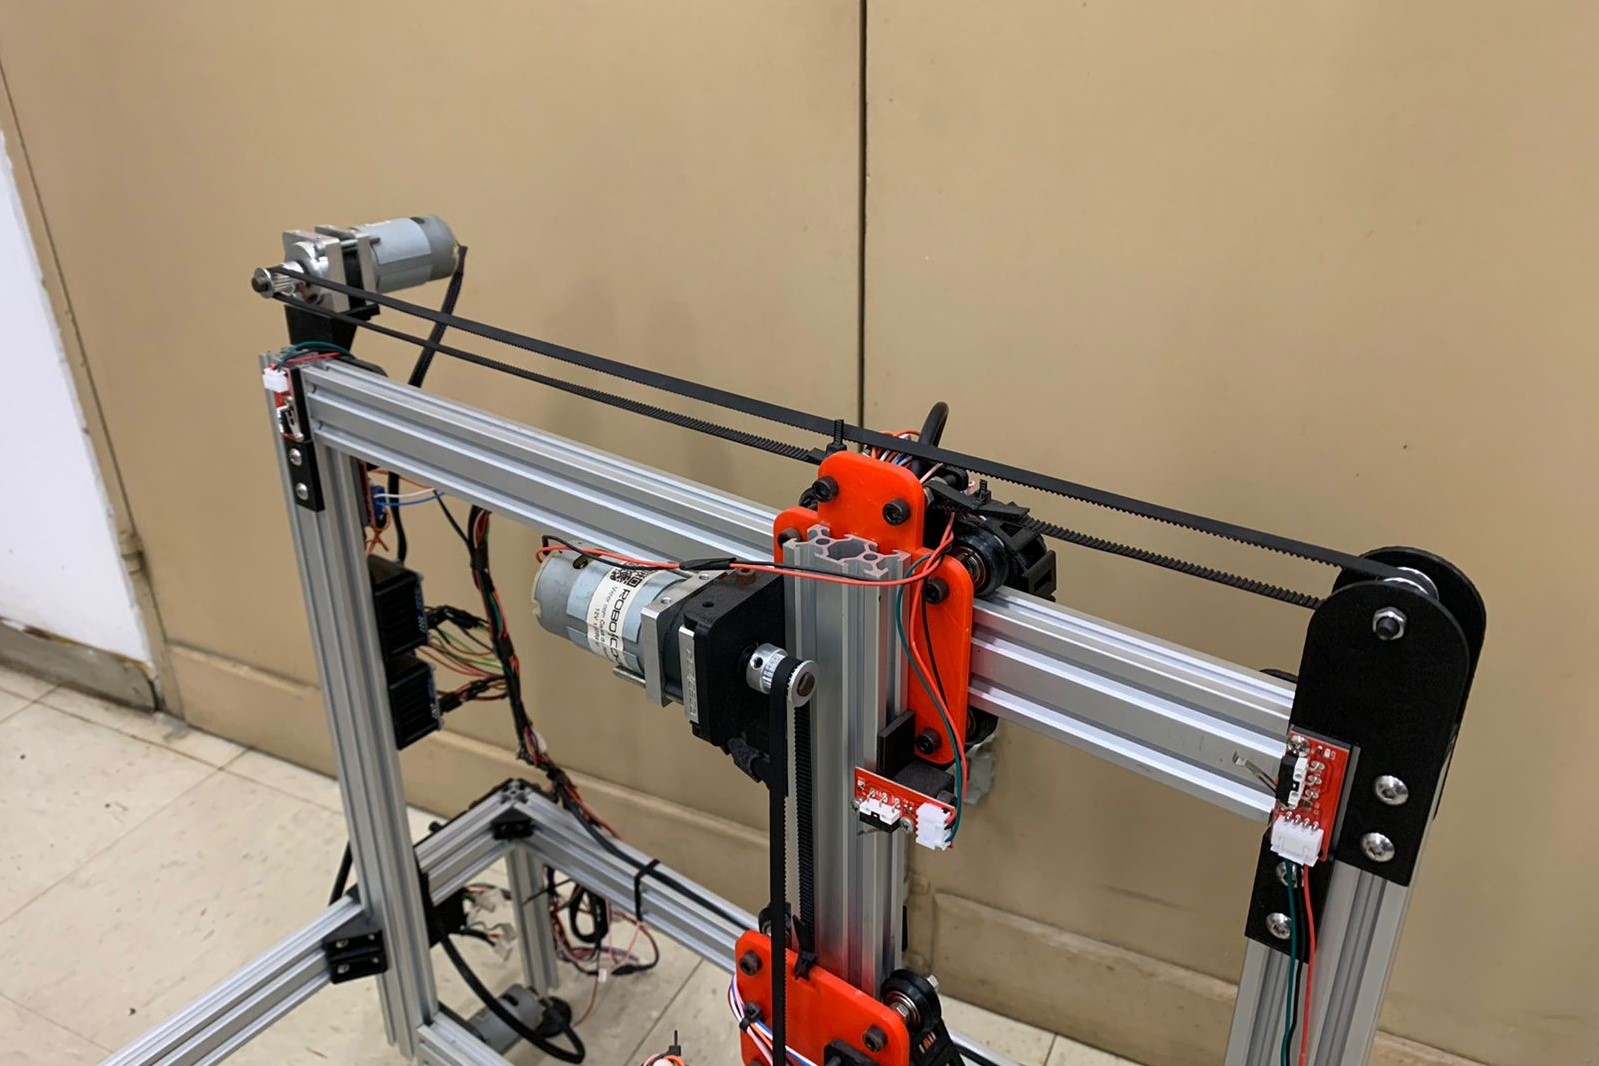
\includegraphics[width=7cm]{images/tração_golgi.jpeg}
        \caption*{Fonte: Autor}
        \label{figura: Esquema de Tração}
        
    \end{minipage}\hfill
    \begin{minipage}{0.5\textwidth}
    
        \centering
        \caption{ Motor com redução}
        \centering % para centralizarmos a figura
        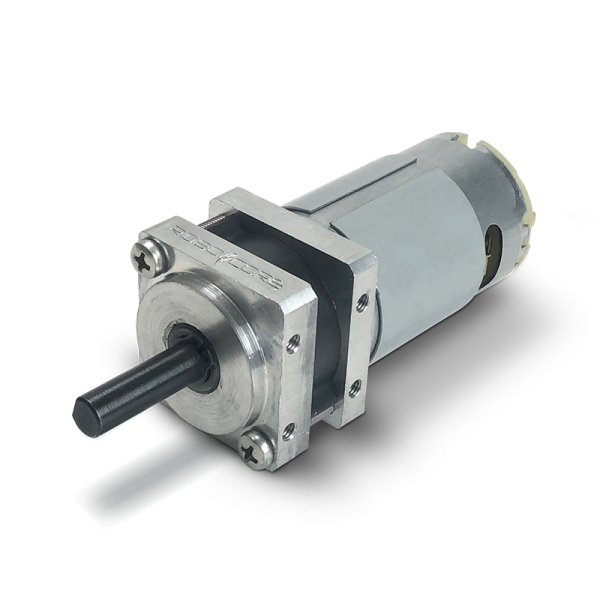
\includegraphics[width=7cm]{images/motor_com_redu.png}
        \caption*{Fonte: Robocore}
        \label{figura: Motor com redução}
        
    \end{minipage}\hfill
\end{figure}

Para captura do remédio, foram usados um atuador linear com uma bomba de vácuo em sua base que permite a sucção do envelope.

\begin{figure}[h]
\centering
    \begin{minipage}{0.5\textwidth}
        \centering
        \caption{Atuador linear}
        \centering % para centralizarmos a figura
        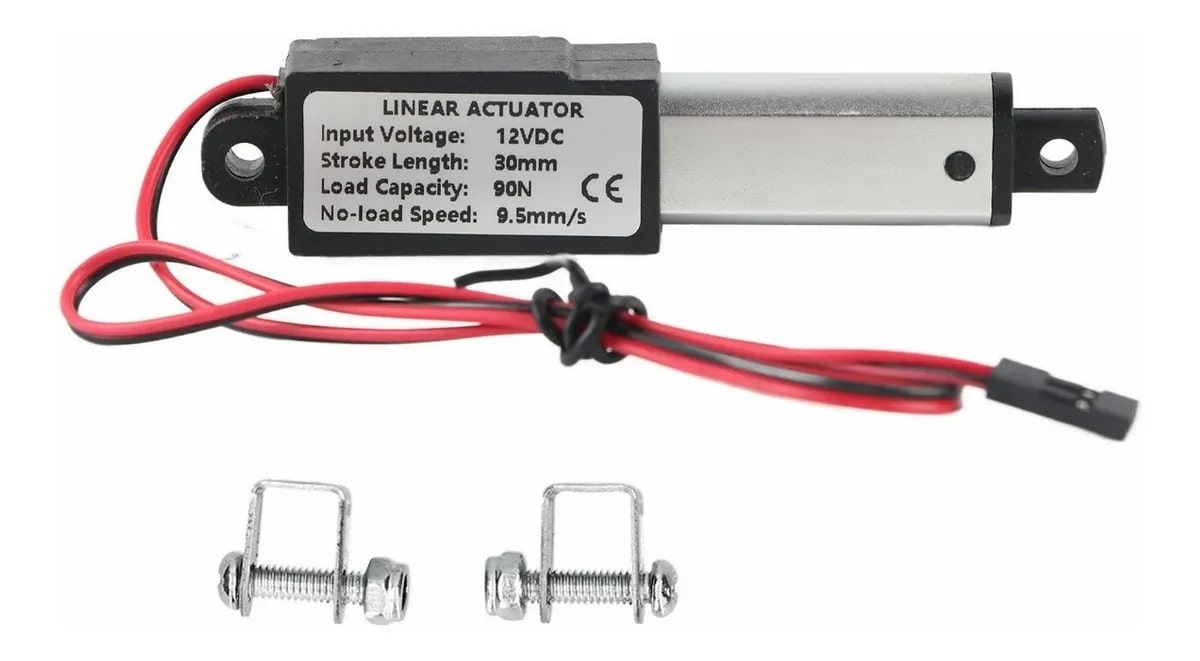
\includegraphics[width=6cm]{images/atuador_linear.jpg}
        \caption*{Fonte: Mercado Livre}
        \label{figura: Atuador}
        
    \end{minipage}\hfill
    \begin{minipage}{0.5\textwidth}
    
        \centering
        \caption{Bomba de vácuo}
        \centering % para centralizarmos a figura
        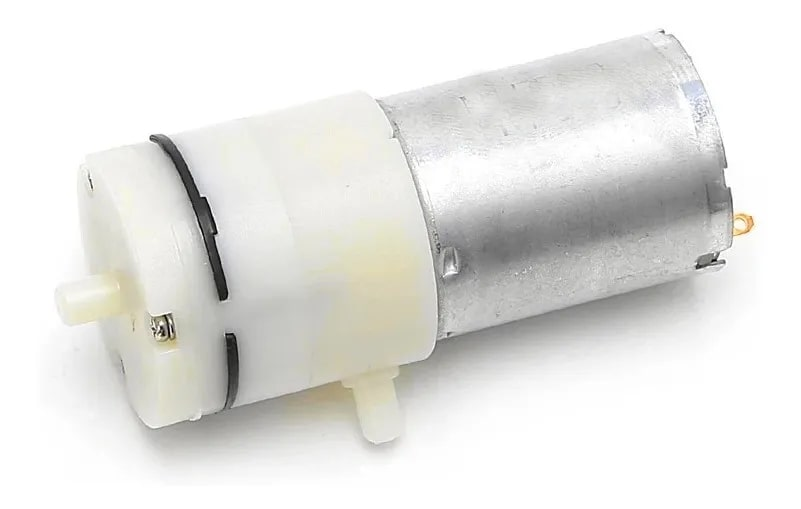
\includegraphics[width=6cm]{images/bomba.jpg}
        \caption*{Fonte: Mercado Livre}
        \label{figura: Bomba de Vácuo}
        
    \end{minipage}\hfill
\end{figure}

\subsection{Carenagem de proteção}

Foi escolhido o Aço inox como material da carenagem de proteção. Para possibilitar a recarga do estoque de remédios foi inserido uma porta de acrílico, que utiliza de travas solenoides e batentes para garantir que a maquina não funcione com a porta aberta, ventoinhas que fornecem pressão positiva para cabine de remdios impedindo a poreira de ser acumulada e garantindo a higiene dos remedios, Foi inserido uma plataforma de controle lateral que permite que o enfermeiro ou farmaceutico opere e a máquina.


\section{Sistemas Eletrônicos}

\subsection{Distribuição de energia}

A distribuição de energia do equipamento pode ser resumida pelo diagrama abaixo. No qual são utilizados de fontes chaveadas, conversores Buck e reguladores internos dos microcontroladores ESP32 e microprocessador Raspberry Pi para a alimentação dos componentes eletrônicos.
\begin{figure}[h]
\centering
    \caption{Distribuição de energia Golgi}
    \centering % para centralizarmos a figura
    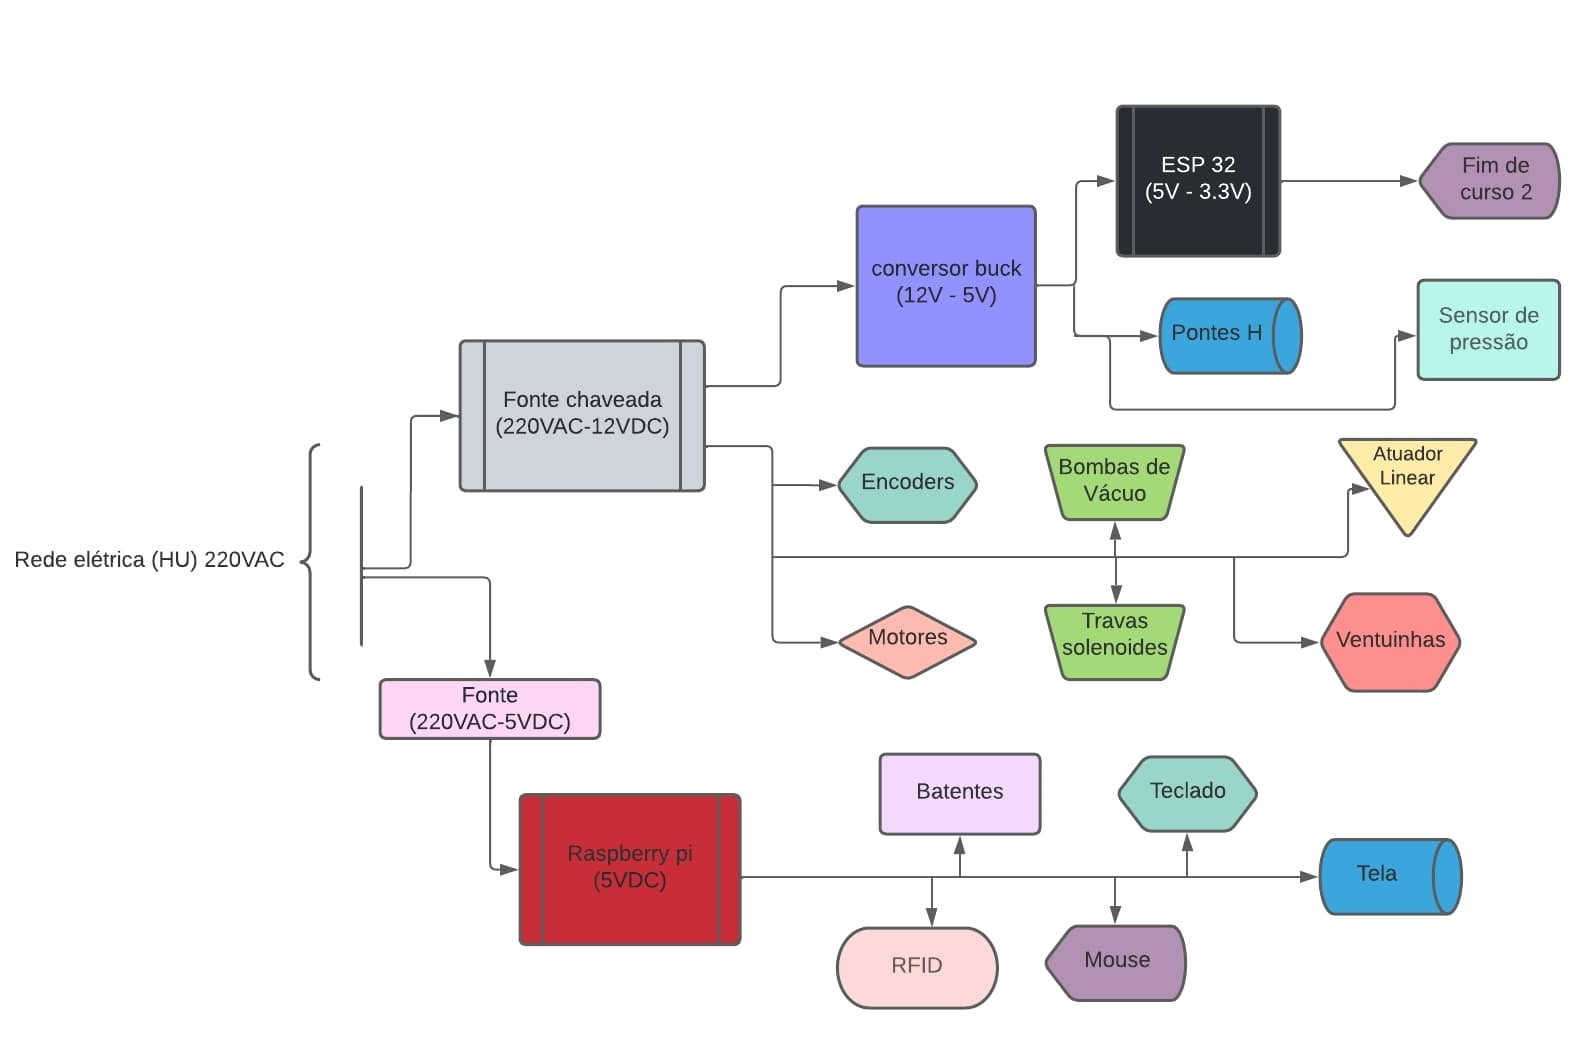
\includegraphics[width=16cm]{images/distribuição_energia_golgi.jpg}
    \caption*{Fonte: Autor}
    \label{figura:distribuição de energia Golgi}
\end{figure}
\begin{figure}[h!]
\centering
    \begin{minipage}{0.3\textwidth}
        \centering
        \caption{Fonte Chaveada 12V}
        \centering % para centralizarmos a figura
        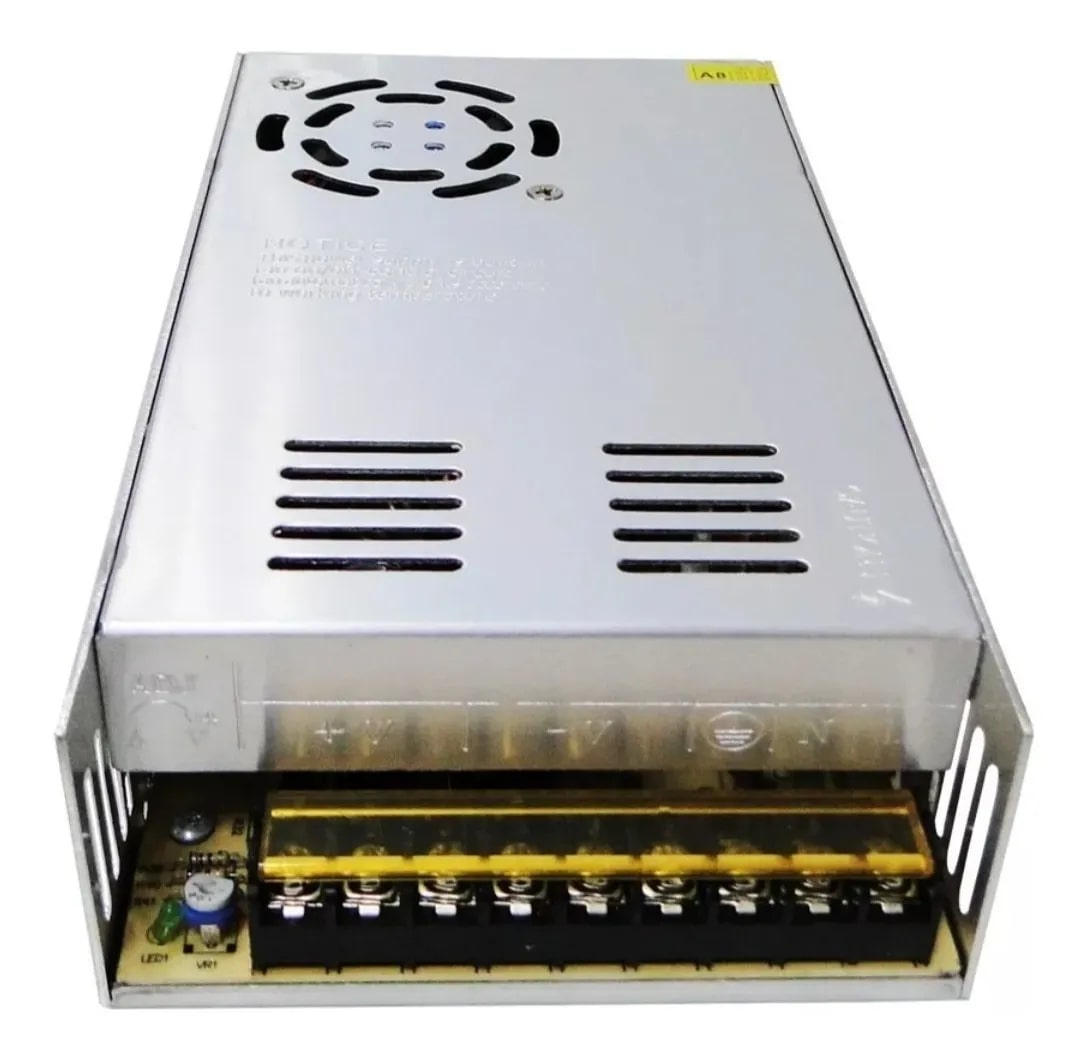
\includegraphics[width=3cm]{images/fonte-chaveada.jpg}
        \caption*{Fonte: Mercado Livre}
        \label{figura: Fonte Chaveada 12V}
        
    \end{minipage}\hfill
    \begin{minipage}{0.3\textwidth}
    
        \centering
        \caption{fonte raspberry pi 3b+}
        \centering % para centralizarmos a figura
        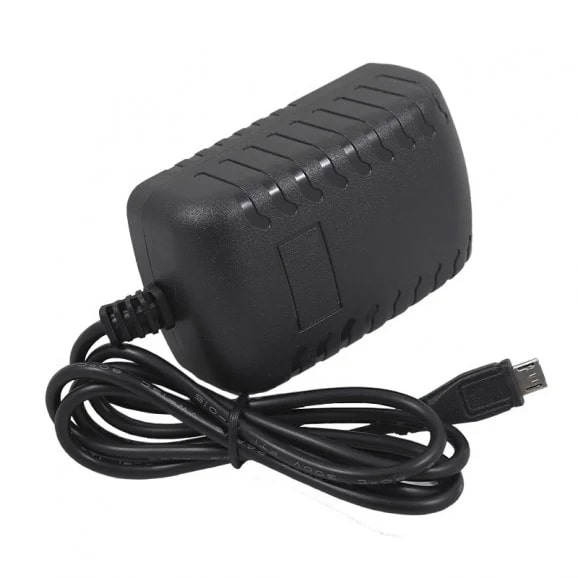
\includegraphics[width=3cm]{images/fonte_rasp.jpg}
        \caption*{Fonte: Mercado Livre}
        \label{figura: fonte raspberry pi 3b+}
        
    \end{minipage}\hfill
    \begin{minipage}{0.3\textwidth}
        \centering
        \caption{Conversor de tensão Buck}
        \centering % para centralizarmos a figura
        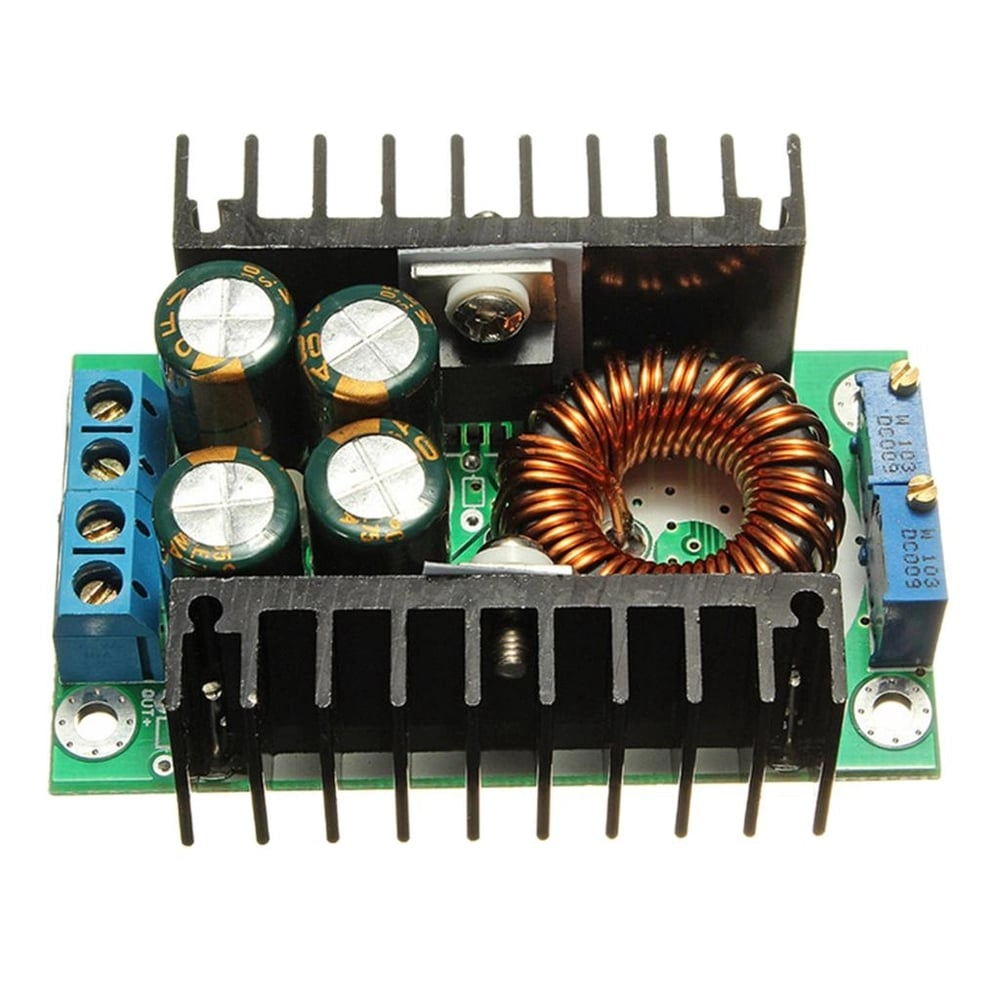
\includegraphics[width=3cm]{images/conversor.jpg}
        \caption*{Fonte: Mercado Livre}
        \label{figura: Conversor de tensão}
        
    \end{minipage}\hfill
\end{figure}
\subsection{Sistema de tração}

Foram escolhidos motores AK555/306PL12S6500C DC escovados para acionar a movimentação, os quais são ativados pela Ponte H BTS 7960 que por sua vez são acionadas via PWM emitido pelo ESP32.Dessa forma controla-se não apenas a direção do movimento como também sua intensidade.
\begin{figure}[h]
\centering
    \begin{minipage}{0.5\textwidth}
        \centering
        \caption{BTS 7960}
        \centering % para centralizarmos a figura
        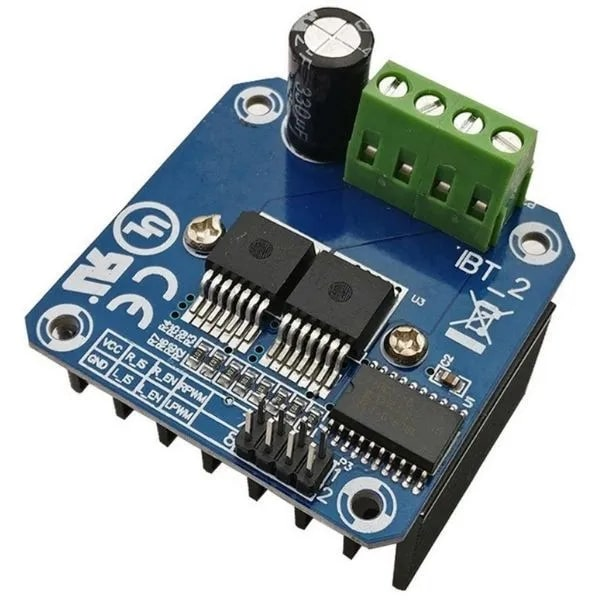
\includegraphics[width=5cm]{images/BTS.jpg}
        \caption*{Fonte: Mercado Livre}
        \label{figura: BTS 7960}
        
    \end{minipage}\hfill
    \begin{minipage}{0.5\textwidth}
    
        \centering
        \caption{AK555}
        \centering % para centralizarmos a figura
        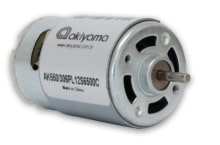
\includegraphics[width=7cm]{images/motor_golgi.jpg}
        \caption*{Fonte: Mercado Livre}
        \label{figura: AK555}
        
    \end{minipage}\hfill
\end{figure}

\subsection{Sistema de realimentação}

Como o sistema de locomoção é baseado em motores DC e não de passo, é necessario um sistema de realimentação e um algoritimo de controle para que seja posssivel ir até a posição desejada. Como sensor de realimentação de posição foram usados encoderes de pulso para mensurar o deslocamento do carrinho e batentes fim de curso para setar os referenciais de inicio e fim do eixo de movimento. Para a checagem da captura é utilizado um sensor de pressão.


\begin{figure}[h]
\centering
    \begin{minipage}{0.3\textwidth}
        \centering
        \caption{Encoder rotativo 600 Pulsos}
        \centering % para centralizarmos a figura
        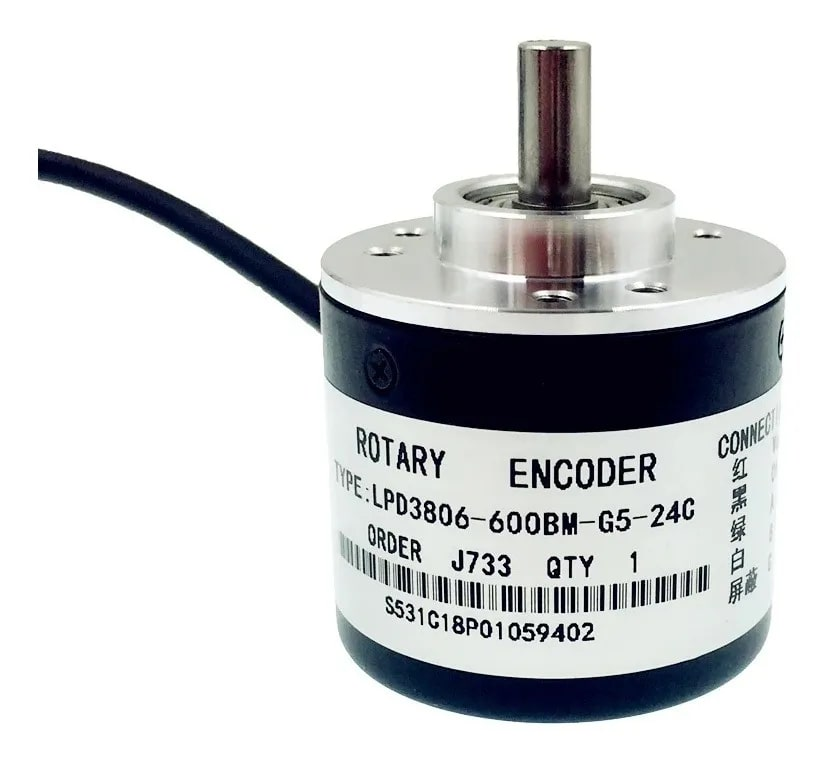
\includegraphics[width=3cm]{images/encoder.jpg}
        \caption*{Fonte: Mercado Livre}
        \label{figura: Encoder rotativo}
        
    \end{minipage}\hfill
    \begin{minipage}{0.3\textwidth}
    
        \centering
        \caption{Sensor de pressão MPX}
        \centering % para centralizarmos a figura
        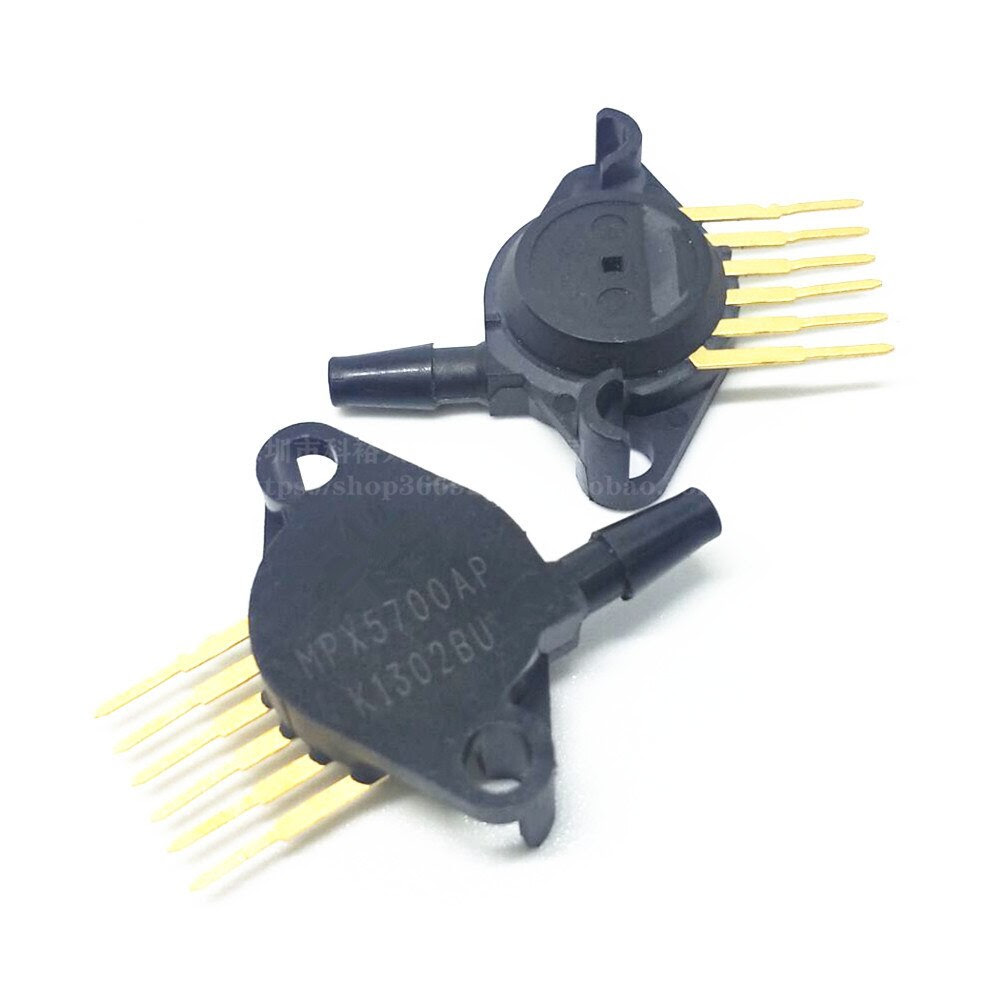
\includegraphics[width=3cm]{images/mpx5700ap.jpg}
        \caption*{Fonte: Mercado Livre}
        \label{figura: Bomba de Vácuo}
        
    \end{minipage}\hfill
    \begin{minipage}{0.3\textwidth}
    
        \centering
        \caption{Módulo chave fim de curso}
        \centering % para centralizarmos a figura
        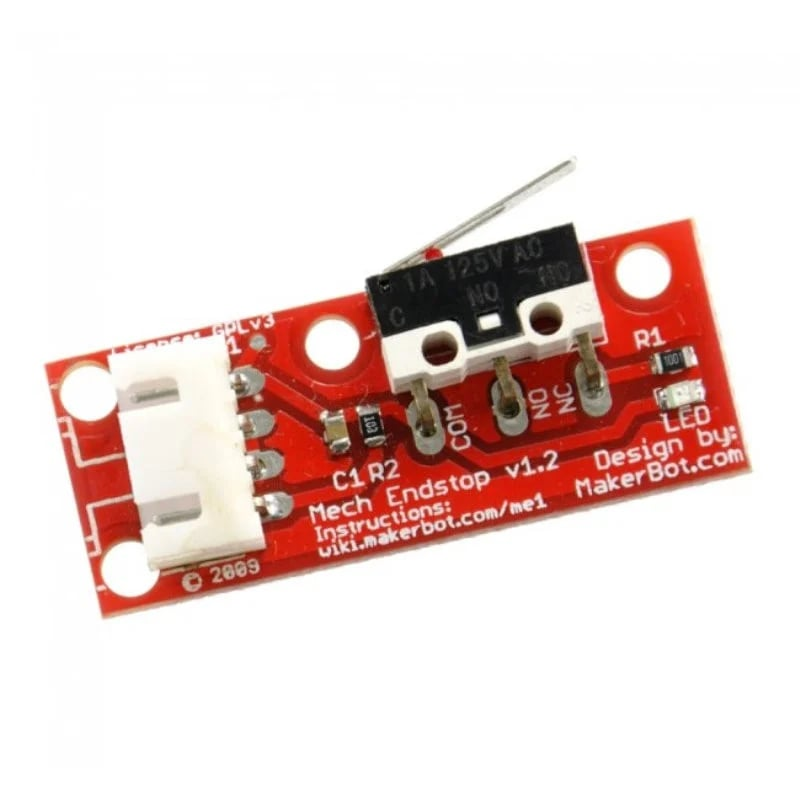
\includegraphics[width=3cm]{images/batente.jpg}
        \caption*{Fonte: Baú da eletrônica}
        \label{figura: Módulo chave fim de curso}
        
        
    \end{minipage}\hfill
\end{figure}

\subsection{Módulos embarcados}

O diagrama abaixo descreve a funcionalida relacionada a cada componente eletrônico. Para garantir essas conexões e separa-las fisicamente de maneira que faça sentido foram desenvolvidos modulos eletronicos, placas de circuito impresso. Essas placas foram feitas no software Altium Designer. 
\begin{figure}[h!]
\centering
    \caption{Eletronica Golgi}
    \centering % para centralizarmos a figura
    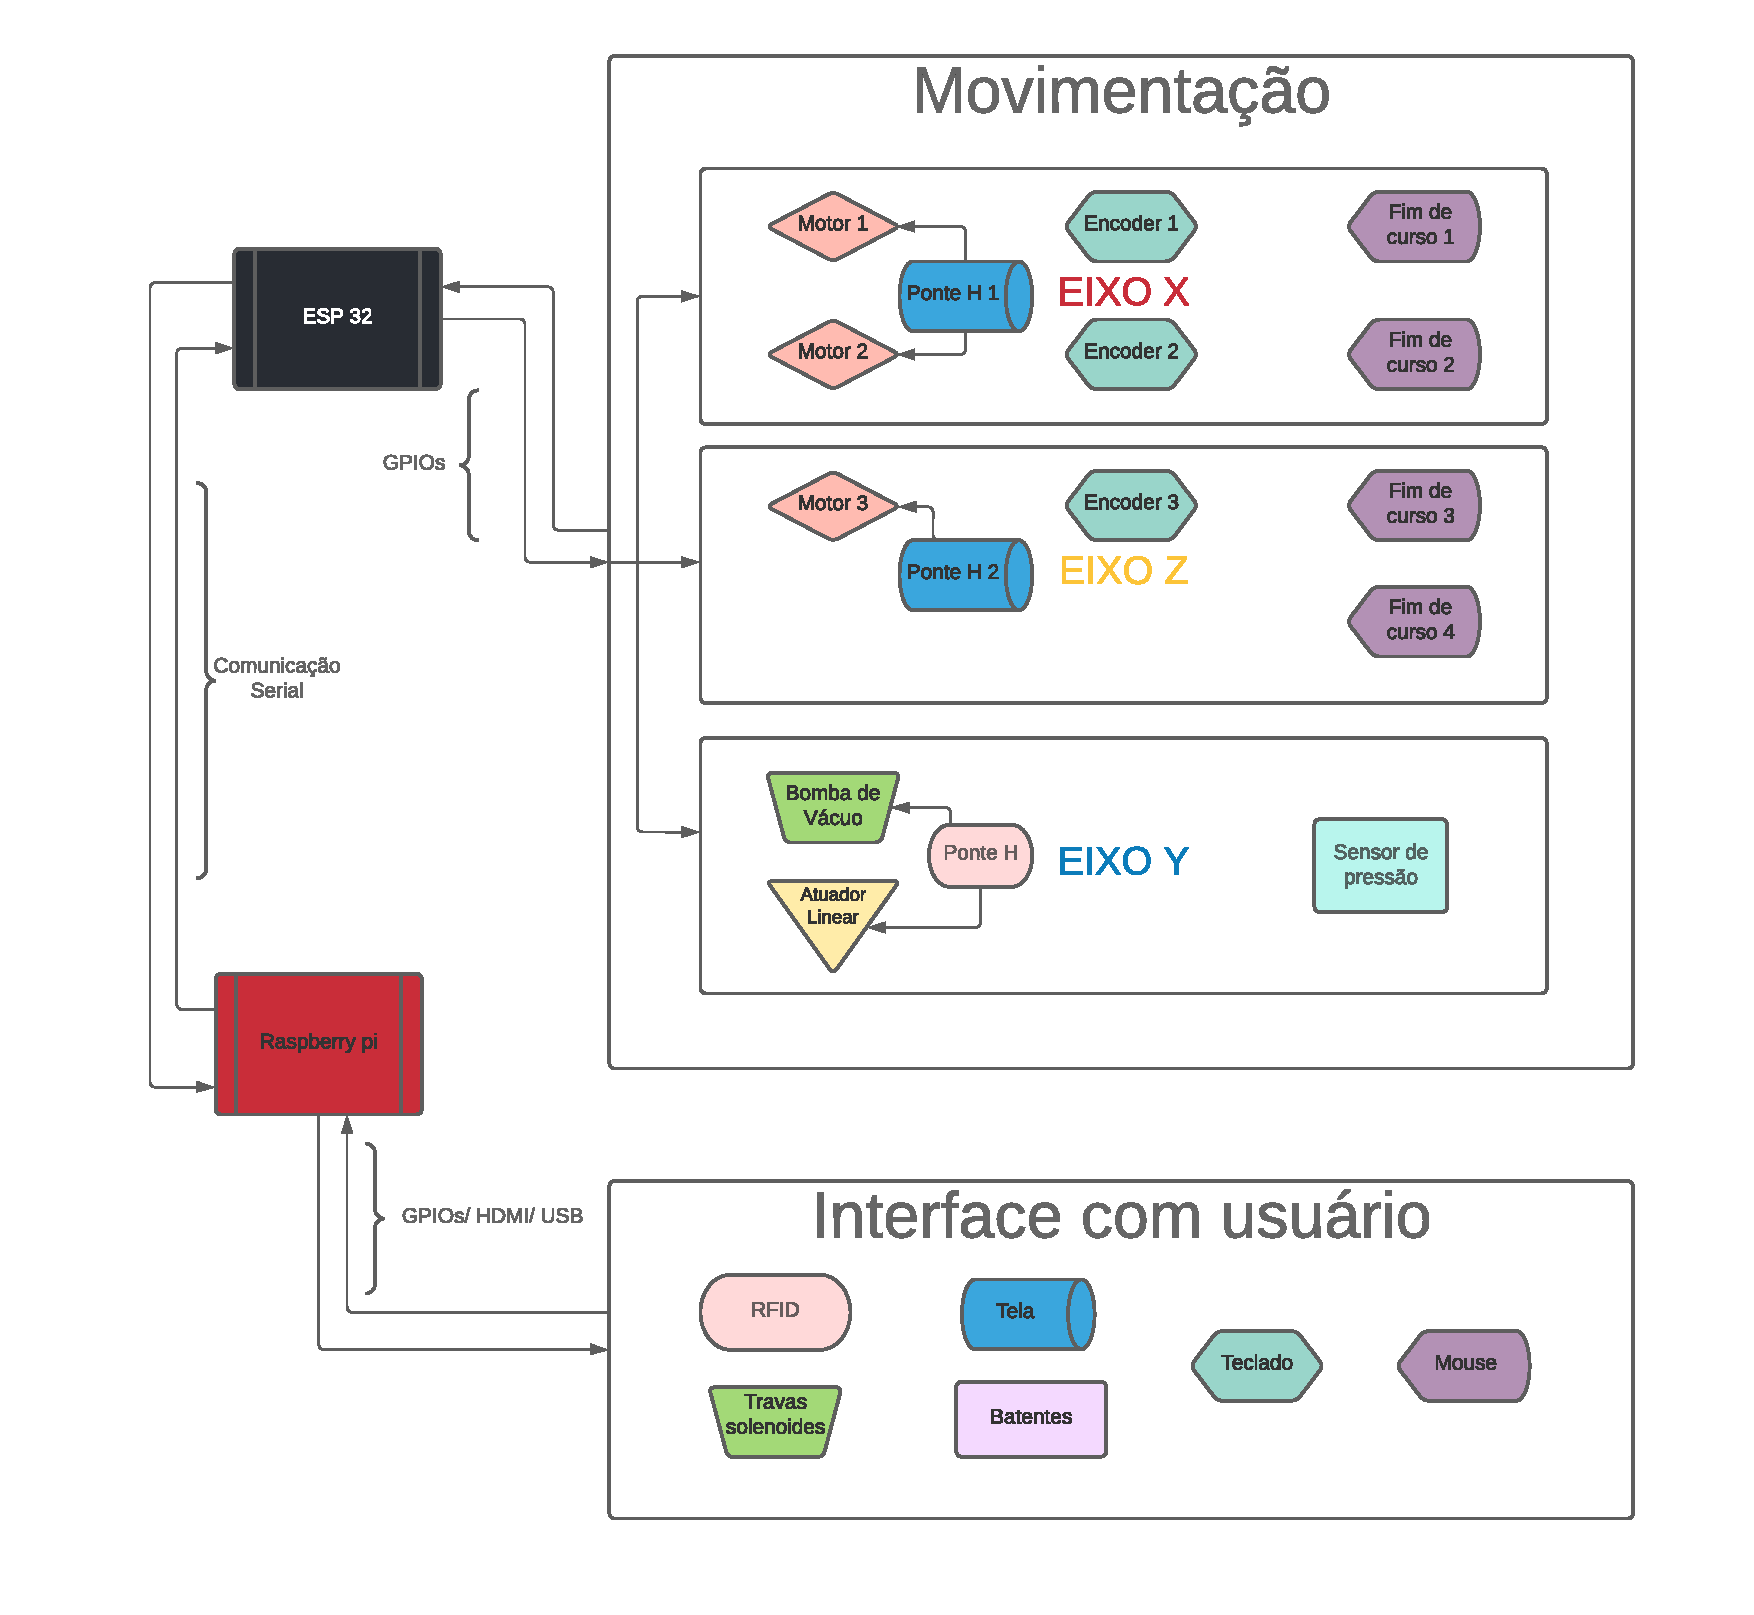
\includegraphics[width=17cm]{images/Eletronica golgi bot (1).pdf}
    \caption*{Fonte: Autor}
    \label{figura:Eletronica Golgi}
\end{figure}


\begin{figure}[h]
\centering
    \begin{minipage}{0.5\textwidth}
        \centering
        \caption{Módulo de movimentação Golgi PCB}
        \centering % para centralizarmos a figura
        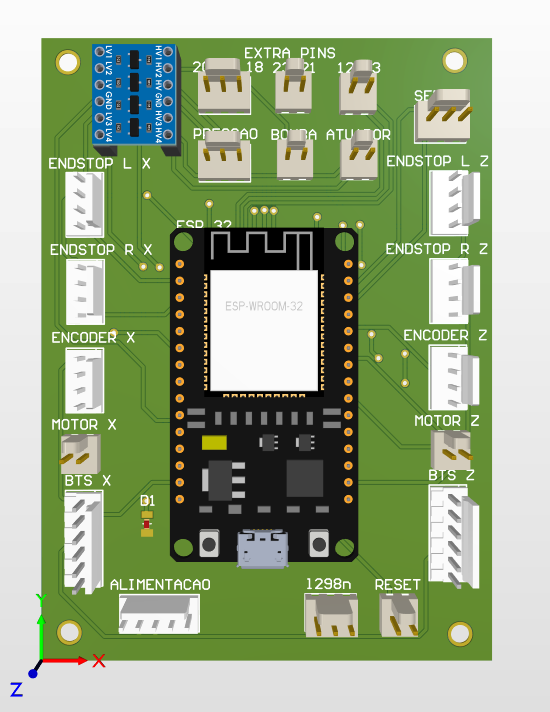
\includegraphics[width=3cm]{images/modulo_movimentação_golgi.png}
        \caption*{Fonte: Autor}
        \label{figura: Módulo de movimentação Golgi PCB}
        
    \end{minipage}\hfill
    \begin{minipage}{0.5\textwidth}
    
        \centering
        \caption{Módulo de movimentação Golgi esquemático}
        \centering % para centralizarmos a figura
        \includegraphics[width=9cm]{images/esquemático_golgi_mov.jpg}
        \caption*{Fonte: Autor}
        \label{figura: Módulo de movimentação Golgi esquemático}
        
    \end{minipage}\hfill
\end{figure}

\begin{figure}[h]
\centering
    \begin{minipage}{0.5\textwidth}
        \centering
        \caption{Módulo Raspberry Golgi PCB}
        \centering % para centralizarmos a figura
        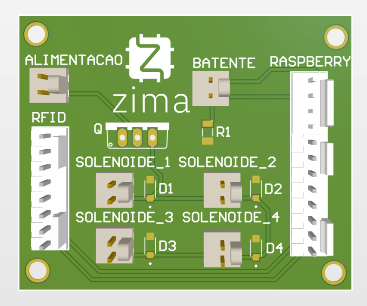
\includegraphics[width=6cm]{images/PCB_rasp.png}
        \caption*{Fonte: Autor}
        \label{figura: Módulo Raspberry Golgi PCB}
        
    \end{minipage}\hfill
    \begin{minipage}{0.5\textwidth}
    
        \centering
        \caption{Módulo Raspberry Golgi esquemático}
        \centering % para centralizarmos a figura
        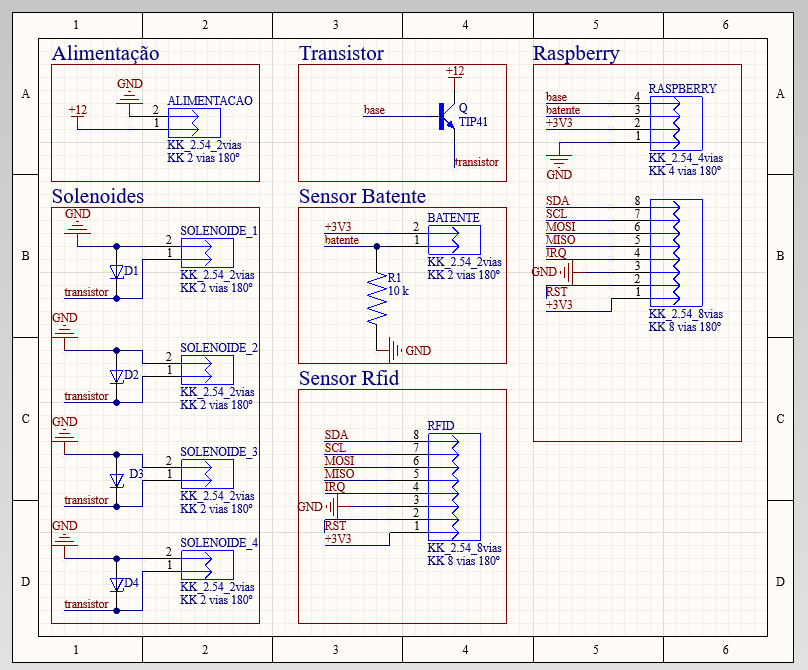
\includegraphics[width=5cm]{images/esqueqmatico_pcb_rasp.png}
        \caption*{Fonte: Autor}
        \label{figura: Módulo Raspberry Golgi esquemático}
        
    \end{minipage}\hfill
\end{figure}

\subsection{Mecanismo de captura}

Para a captura do remédio foram utilizados dois motor, um na forma de bomba de vácuo e outro em um atuador linear. Ambos são controlados pela ponte H l289n que permite controlar a extensão e contração bem como o acionamento da bomba através de pinos digitais do ESP-32.



\begin{figure}[h]
\centering
    \begin{minipage}{0.3\textwidth}
        \centering
        \caption{Atuador linear}
        \centering % para centralizarmos a figura
        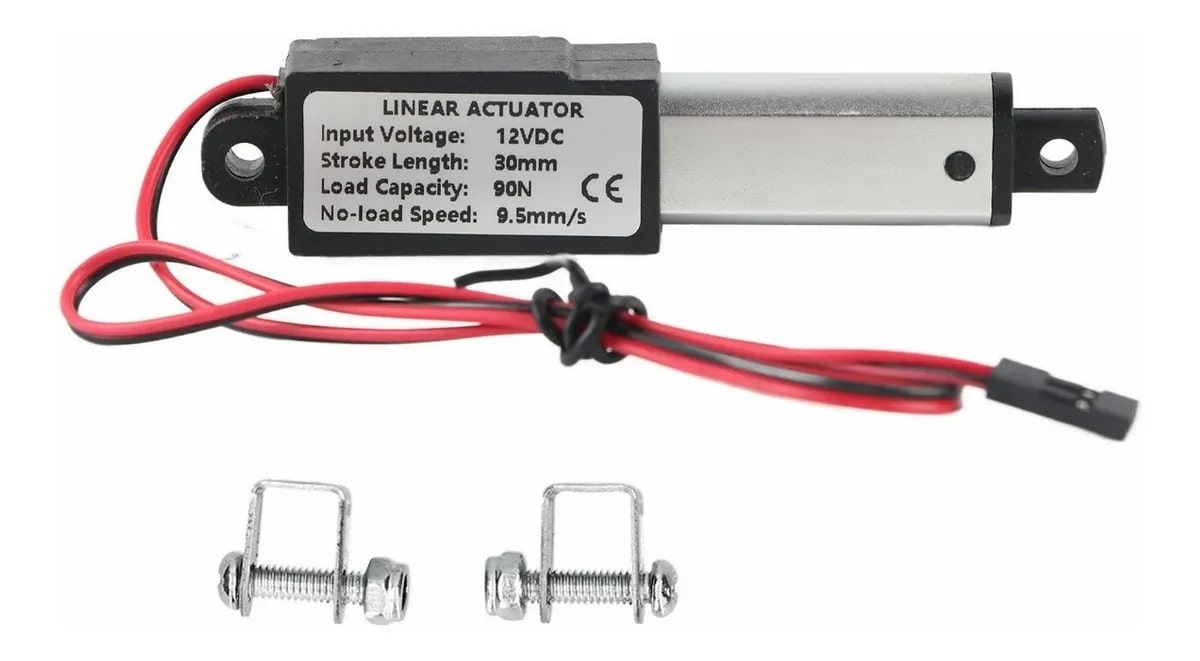
\includegraphics[width=3cm]{images/atuador_linear.jpg}
        \caption*{Fonte: Mercado Livre}
        \label{figura: Atuador}
        
    \end{minipage}\hfill
    \begin{minipage}{0.3\textwidth}
    
        \centering
        \caption{Bomba de vácuo}
        \centering % para centralizarmos a figura
        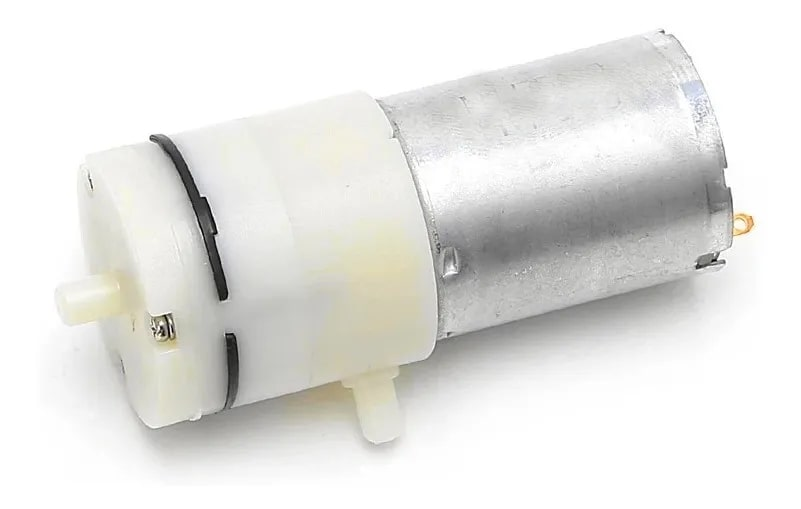
\includegraphics[width=5cm]{images/bomba.jpg}
        \caption*{Fonte: Mercado Livre}
        \label{figura: Bomba de Vácuo}
        
    \end{minipage}\hfill
    \begin{minipage}{0.3\textwidth}
        \centering
        \caption{Ponte H l298n}
        \centering % para centralizarmos a figura
        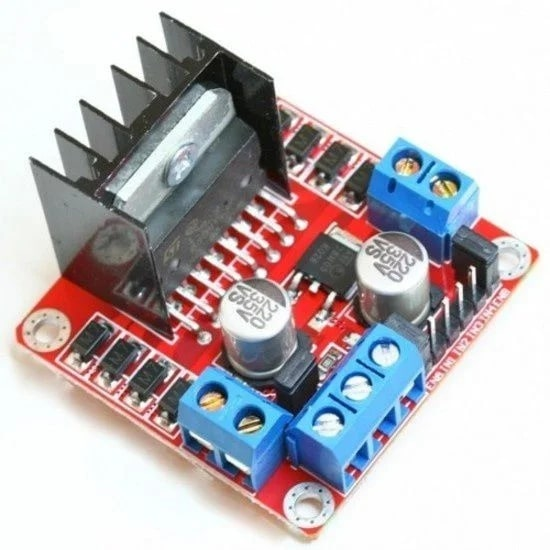
\includegraphics[width=3cm]{images/l298n.jpg}
        \caption*{Fonte: Mercado Livre}
        \label{figura: l298n}
        
    \end{minipage}\hfill
\end{figure}


\end{document}